\documentclass{book}
\usepackage[a4paper,top=2.5cm,bottom=2.5cm,left=2.5cm,right=2.5cm]{geometry}
\usepackage{makeidx}
\usepackage{natbib}
\usepackage{graphicx}
\usepackage{multicol}
\usepackage{float}
\usepackage{listings}
\usepackage{color}
\usepackage{ifthen}
\usepackage[table]{xcolor}
\usepackage{textcomp}
\usepackage{alltt}
\usepackage{ifpdf}
\ifpdf
\usepackage[pdftex,
            pagebackref=true,
            colorlinks=true,
            linkcolor=blue,
            unicode
           ]{hyperref}
\else
\usepackage[ps2pdf,
            pagebackref=true,
            colorlinks=true,
            linkcolor=blue,
            unicode
           ]{hyperref}
\usepackage{pspicture}
\fi
\usepackage[utf8]{inputenc}
\usepackage{mathptmx}
\usepackage[scaled=.90]{helvet}
\usepackage{courier}
\usepackage{sectsty}
\usepackage{amssymb}
\usepackage[titles]{tocloft}
\usepackage{doxygen}
\lstset{language=C++,inputencoding=utf8,basicstyle=\footnotesize,breaklines=true,breakatwhitespace=true,tabsize=4,numbers=left }
\makeindex
\setcounter{tocdepth}{3}
\renewcommand{\footrulewidth}{0.4pt}
\renewcommand{\familydefault}{\sfdefault}
\hfuzz=15pt
\setlength{\emergencystretch}{15pt}
\hbadness=750
\tolerance=750
\begin{document}
\hypersetup{pageanchor=false,citecolor=blue}
\begin{titlepage}
\vspace*{7cm}
\begin{center}
{\Large pygeors \\[1ex]\large 0.\-1 }\\
\vspace*{1cm}
{\large Generated by Doxygen 1.8.3.1}\\
\vspace*{0.5cm}
{\small Mon Jan 21 2013 18:02:51}\\
\end{center}
\end{titlepage}
\clearemptydoublepage
\pagenumbering{roman}
\tableofcontents
\clearemptydoublepage
\pagenumbering{arabic}
\hypersetup{pageanchor=true,citecolor=blue}
\chapter{Namespace Index}
\section{Namespace List}
Here is a list of all documented namespaces with brief descriptions\-:\begin{DoxyCompactList}
\item\contentsline{section}{\hyperlink{namespacegeors}{geors} \\*Name\-: geors.\-py Purpose\-: Geoinformation for D\-E based on opengeodb data and openstreetmap webservice Author\-: \href{mailto:burger@burgerdev.de}{\tt burger@burgerdev.\-de} Created\-: 08.\-01.\-2013 Copyright\-: (c) Markus Döring 2013, plz.\-db is in the public domain (thanks to opengeodb.\-org) full text search results are covered by the Database Contents License (Db\-C\-L) 1.\-0 Licence\-: G\-P\-L3, O\-Db\-L (see openstreetmap.\-org for details) }{\pageref{namespacegeors}}{}
\end{DoxyCompactList}

\chapter{Hierarchical Index}
\section{Class Hierarchy}
This inheritance list is sorted roughly, but not completely, alphabetically\-:\begin{DoxyCompactList}
\item object\begin{DoxyCompactList}
\item \contentsline{section}{geors.\-Geo\-Loc}{\pageref{classgeors_1_1GeoLoc}}{}
\end{DoxyCompactList}
\end{DoxyCompactList}

\chapter{Class Index}
\section{Class List}
Here are the classes, structs, unions and interfaces with brief descriptions\-:\begin{DoxyCompactList}
\item\contentsline{section}{\hyperlink{classgeors_1_1GeoLoc}{geors.\-Geo\-Loc} \\*Geographic location object }{\pageref{classgeors_1_1GeoLoc}}{}
\end{DoxyCompactList}

\chapter{Namespace Documentation}
\hypertarget{namespacegeors}{\section{geors Namespace Reference}
\label{namespacegeors}\index{geors@{geors}}
}


Name\-: geors.\-py Purpose\-: Geoinformation for D\-E based on opengeodb data and openstreetmap webservice Author\-: \href{mailto:burger@burgerdev.de}{\tt burger@burgerdev.\-de} Created\-: 08.\-01.\-2013 Copyright\-: (c) Markus Döring 2013, plz.\-db is in the public domain (thanks to opengeodb.\-org) full text search results are covered by the Database Contents License (Db\-C\-L) 1.\-0 Licence\-: G\-P\-L3, O\-Db\-L (see openstreetmap.\-org for details)  


\subsection*{Classes}
\begin{DoxyCompactItemize}
\item 
class \hyperlink{classgeors_1_1GeoLoc}{Geo\-Loc}
\begin{DoxyCompactList}\small\item\em geographic location object \end{DoxyCompactList}\end{DoxyCompactItemize}
\subsection*{Functions}
\begin{DoxyCompactItemize}
\item 
def \hyperlink{namespacegeors_a524e72573297cfd02214f0ee5c416330}{gcd}
\begin{DoxyCompactList}\small\item\em great circle distance \end{DoxyCompactList}\item 
def \hyperlink{namespacegeors_a250a82f910c096532544fbe6b5a3f808}{distance}
\begin{DoxyCompactList}\small\item\em calculate distance between Geo\-Locs \end{DoxyCompactList}\item 
def \hyperlink{namespacegeors_abf605583f4b44d3ade8ac9a0a9da63d1}{area}
\begin{DoxyCompactList}\small\item\em get surrounding Geo\-Locs \end{DoxyCompactList}\end{DoxyCompactItemize}
\subsection*{Variables}
\begin{DoxyCompactItemize}
\item 
\hypertarget{namespacegeors_a8b633d071062d35496cc4c35670725de}{tuple {\bfseries \-\_\-conn} = sqlite3.\-connect(os.\-path.\-join(os.\-path.\-dirname( \-\_\-\-\_\-file\-\_\-\-\_\- ), 'plz.\-db'))}\label{namespacegeors_a8b633d071062d35496cc4c35670725de}

\item 
\hypertarget{namespacegeors_ac1a31bbbc06a9fd9bfdc8860c3a61e0c}{string \hyperlink{namespacegeors_ac1a31bbbc06a9fd9bfdc8860c3a61e0c}{osm\-\_\-useragent} = \char`\"{}pygeors -\/ autocompletion\char`\"{}}\label{namespacegeors_ac1a31bbbc06a9fd9bfdc8860c3a61e0c}

\begin{DoxyCompactList}\small\item\em openstreetmap user agent set this to your app's name \end{DoxyCompactList}\item 
\hypertarget{namespacegeors_a61e250eb73c709b7c855e9e96b0a3fcd}{\hyperlink{namespacegeors_a61e250eb73c709b7c855e9e96b0a3fcd}{osm\-\_\-email} = None}\label{namespacegeors_a61e250eb73c709b7c855e9e96b0a3fcd}

\begin{DoxyCompactList}\small\item\em openstreetmap email address provide an email address for O\-S\-M to contact you \end{DoxyCompactList}\item 
\hypertarget{namespacegeors_a2ab76ea44ea2c03066064d65ea4fb76e}{tuple {\bfseries \-\_\-a} = \hyperlink{classgeors_1_1GeoLoc}{Geo\-Loc}()}\label{namespacegeors_a2ab76ea44ea2c03066064d65ea4fb76e}

\item 
\hypertarget{namespacegeors_a9e2bf8a114400d8ee4b119082f45aebf}{tuple {\bfseries \-\_\-b} = \hyperlink{classgeors_1_1GeoLoc}{Geo\-Loc}()}\label{namespacegeors_a9e2bf8a114400d8ee4b119082f45aebf}

\item 
\hypertarget{namespacegeors_a3a65fd9ccc9e58725c7b9ffbb40081b2}{tuple {\bfseries \-\_\-c} = \hyperlink{classgeors_1_1GeoLoc}{Geo\-Loc}()}\label{namespacegeors_a3a65fd9ccc9e58725c7b9ffbb40081b2}

\item 
\hypertarget{namespacegeors_ab886686d60b4ac319f24920edbdb2599}{tuple {\bfseries \-\_\-d} = \hyperlink{namespacegeors_abf605583f4b44d3ade8ac9a0a9da63d1}{area}(\-\_\-c,10)}\label{namespacegeors_ab886686d60b4ac319f24920edbdb2599}

\item 
\hypertarget{namespacegeors_a9da4cdb2d911e48be522d7998e37469a}{tuple {\bfseries \-\_\-e} = \hyperlink{namespacegeors_a250a82f910c096532544fbe6b5a3f808}{distance}(\-\_\-c,\-\_\-d)}\label{namespacegeors_a9da4cdb2d911e48be522d7998e37469a}

\item 
\hypertarget{namespacegeors_a3c2341af5962793f6c8bb26e0f454b0b}{tuple {\bfseries \-\_\-g} = \hyperlink{classgeors_1_1GeoLoc}{Geo\-Loc}()}\label{namespacegeors_a3c2341af5962793f6c8bb26e0f454b0b}

\end{DoxyCompactItemize}


\subsection{Detailed Description}
Name\-: geors.\-py Purpose\-: Geoinformation for D\-E based on opengeodb data and openstreetmap webservice Author\-: \href{mailto:burger@burgerdev.de}{\tt burger@burgerdev.\-de} Created\-: 08.\-01.\-2013 Copyright\-: (c) Markus Döring 2013, plz.\-db is in the public domain (thanks to opengeodb.\-org) full text search results are covered by the Database Contents License (Db\-C\-L) 1.\-0 Licence\-: G\-P\-L3, O\-Db\-L (see openstreetmap.\-org for details) 

\subsection{Function Documentation}
\hypertarget{namespacegeors_abf605583f4b44d3ade8ac9a0a9da63d1}{\index{geors@{geors}!area@{area}}
\index{area@{area}!geors@{geors}}
\subsubsection[{area}]{\setlength{\rightskip}{0pt plus 5cm}def geors.\-area (
\begin{DoxyParamCaption}
\item[{}]{loc, }
\item[{}]{dist}
\end{DoxyParamCaption}
)}}\label{namespacegeors_abf605583f4b44d3ade8ac9a0a9da63d1}


get surrounding Geo\-Locs 


\begin{DoxyParams}{Parameters}
{\em loc} & a \hyperlink{classgeors_1_1GeoLoc}{Geo\-Loc} obejct to start with \\
\hline
{\em dist} & a distance in kilometres to search in \\
\hline
\end{DoxyParams}
\begin{DoxyReturn}{Returns}
a list of Geo\-Locs (aka cities) within the specified radius of loc
\end{DoxyReturn}
usage (and doctests)\-:

\begin{quotation}
\begin{quotation}
\begin{quotation}
area(\-None, 0)

g = \hyperlink{classgeors_1_1GeoLoc}{Geo\-Loc}(\mbox{[}87527, \char`\"{}\-Sonthofen\char`\"{}, None, None, \char`\"{}87527\char`\"{}\mbox{]}) L = area(g,0.\-1) len(\-L)

\end{quotation}


\end{quotation}


\end{quotation}
1 \begin{quotation}
\begin{quotation}
\begin{quotation}
L\mbox{[}0\mbox{]}.zipcode

\end{quotation}


\end{quotation}


\end{quotation}
'87527' \hypertarget{namespacegeors_a250a82f910c096532544fbe6b5a3f808}{\index{geors@{geors}!distance@{distance}}
\index{distance@{distance}!geors@{geors}}
\subsubsection[{distance}]{\setlength{\rightskip}{0pt plus 5cm}def geors.\-distance (
\begin{DoxyParamCaption}
\item[{}]{loc, }
\item[{}]{locs}
\end{DoxyParamCaption}
)}}\label{namespacegeors_a250a82f910c096532544fbe6b5a3f808}


calculate distance between Geo\-Locs 


\begin{DoxyParams}{Parameters}
{\em loc} & a \hyperlink{classgeors_1_1GeoLoc}{Geo\-Loc} obejct to start with \\
\hline
{\em locs} & either a \hyperlink{classgeors_1_1GeoLoc}{Geo\-Loc} object or a list of \hyperlink{classgeors_1_1GeoLoc}{Geo\-Loc} objects \\
\hline
\end{DoxyParams}
\begin{DoxyReturn}{Returns}
a float or a list of floats (depending on the input) with the distance in kilometres
\end{DoxyReturn}
usage (and doctests)\-:

\begin{quotation}
\begin{quotation}
\begin{quotation}
distance(\-None, None)

distance(\-None, \mbox{[}\-None, None\mbox{]})

\end{quotation}


\end{quotation}


\end{quotation}
\mbox{[}None, None\mbox{]} \hypertarget{namespacegeors_a524e72573297cfd02214f0ee5c416330}{\index{geors@{geors}!gcd@{gcd}}
\index{gcd@{gcd}!geors@{geors}}
\subsubsection[{gcd}]{\setlength{\rightskip}{0pt plus 5cm}def geors.\-gcd (
\begin{DoxyParamCaption}
\item[{}]{lat1, }
\item[{}]{lon1, }
\item[{}]{lat2, }
\item[{}]{lon2, }
\item[{}]{r = {\ttfamily 6367.5}}
\end{DoxyParamCaption}
)}}\label{namespacegeors_a524e72573297cfd02214f0ee5c416330}


great circle distance 

compute the great circle distance between two latitude/longitude pairs 
\begin{DoxyParams}{Parameters}
{\em lat1} & first latitude \\
\hline
{\em lon1} & first longitude \\
\hline
{\em lat2} & second latitude \\
\hline
{\em lon2} & second longitude \\
\hline
{\em r} & radius (defalut\-: earth radius in km)\\
\hline
\end{DoxyParams}
\begin{DoxyReturn}{Returns}
distance between the coordinates, units are the same as in the input 
\end{DoxyReturn}

\chapter{Class Documentation}
\hypertarget{classgeors_1_1GeoLoc}{\section{geors.\-Geo\-Loc Class Reference}
\label{classgeors_1_1GeoLoc}\index{geors.\-Geo\-Loc@{geors.\-Geo\-Loc}}
}


geographic location object  


Inheritance diagram for geors.\-Geo\-Loc\-:\begin{figure}[H]
\begin{center}
\leavevmode
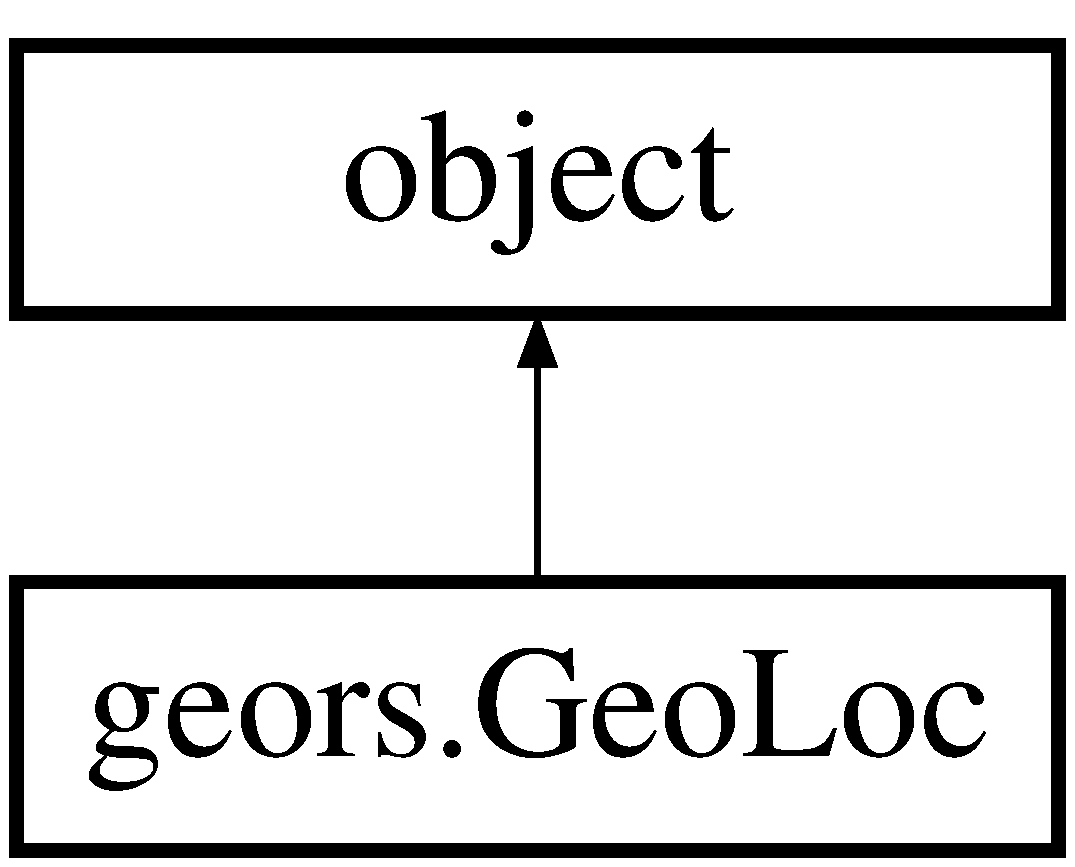
\includegraphics[height=2.000000cm]{classgeors_1_1GeoLoc}
\end{center}
\end{figure}
\subsection*{Public Member Functions}
\begin{DoxyCompactItemize}
\item 
def \hyperlink{classgeors_1_1GeoLoc_aec420200a480eb3edc214ec6c25c980e}{\-\_\-\-\_\-init\-\_\-\-\_\-}
\begin{DoxyCompactList}\small\item\em the constructor \end{DoxyCompactList}\item 
\hypertarget{classgeors_1_1GeoLoc_af9fe7d2b66ce73ee115d211c99c18db0}{def \hyperlink{classgeors_1_1GeoLoc_af9fe7d2b66ce73ee115d211c99c18db0}{\-\_\-\-\_\-str\-\_\-\-\_\-}}\label{classgeors_1_1GeoLoc_af9fe7d2b66ce73ee115d211c99c18db0}

\begin{DoxyCompactList}\small\item\em convert to string \end{DoxyCompactList}\item 
def \hyperlink{classgeors_1_1GeoLoc_ad60e96d584d8aa6039ca7deb533f051e}{complete}
\begin{DoxyCompactList}\small\item\em look up \hyperlink{classgeors_1_1GeoLoc}{Geo\-Loc} information Complete the geographic information in this \hyperlink{classgeors_1_1GeoLoc}{Geo\-Loc} object. \end{DoxyCompactList}\end{DoxyCompactItemize}
\subsection*{Public Attributes}
\begin{DoxyCompactItemize}
\item 
\hypertarget{classgeors_1_1GeoLoc_a61510b2a72e53f080eb4577a93a5544f}{\hyperlink{classgeors_1_1GeoLoc_a61510b2a72e53f080eb4577a93a5544f}{city}}\label{classgeors_1_1GeoLoc_a61510b2a72e53f080eb4577a93a5544f}

\begin{DoxyCompactList}\small\item\em the city (string, default\-: None) \end{DoxyCompactList}\item 
\hypertarget{classgeors_1_1GeoLoc_a0d6a0704ea6b37dae91fceb128363122}{\hyperlink{classgeors_1_1GeoLoc_a0d6a0704ea6b37dae91fceb128363122}{zipcode}}\label{classgeors_1_1GeoLoc_a0d6a0704ea6b37dae91fceb128363122}

\begin{DoxyCompactList}\small\item\em the zip code (string, default\-: None) \end{DoxyCompactList}\item 
\hypertarget{classgeors_1_1GeoLoc_ab3c4d764d152b0aa73c766a3e8b85907}{\hyperlink{classgeors_1_1GeoLoc_ab3c4d764d152b0aa73c766a3e8b85907}{county}}\label{classgeors_1_1GeoLoc_ab3c4d764d152b0aa73c766a3e8b85907}

\begin{DoxyCompactList}\small\item\em the county (string, default\-: None) \end{DoxyCompactList}\item 
\hypertarget{classgeors_1_1GeoLoc_a65a154050406aad462d1f858332c28ba}{\hyperlink{classgeors_1_1GeoLoc_a65a154050406aad462d1f858332c28ba}{state}}\label{classgeors_1_1GeoLoc_a65a154050406aad462d1f858332c28ba}

\begin{DoxyCompactList}\small\item\em the state (string, default\-: None) \end{DoxyCompactList}\item 
\hypertarget{classgeors_1_1GeoLoc_a2d03502d18afd8b1e4a7802f71ef9a32}{\hyperlink{classgeors_1_1GeoLoc_a2d03502d18afd8b1e4a7802f71ef9a32}{country}}\label{classgeors_1_1GeoLoc_a2d03502d18afd8b1e4a7802f71ef9a32}

\begin{DoxyCompactList}\small\item\em the country (string, default\-: \char`\"{}\-Deutschland\char`\"{}) \end{DoxyCompactList}\item 
\hypertarget{classgeors_1_1GeoLoc_a0b8b5771e4e55088bf84e2e112c95c0e}{\hyperlink{classgeors_1_1GeoLoc_a0b8b5771e4e55088bf84e2e112c95c0e}{countrycode}}\label{classgeors_1_1GeoLoc_a0b8b5771e4e55088bf84e2e112c95c0e}

\begin{DoxyCompactList}\small\item\em the countrycode, in most cases T\-L\-D (string, default\-: \char`\"{}de\char`\"{}) \end{DoxyCompactList}\item 
\hypertarget{classgeors_1_1GeoLoc_a3f6c5595b27d72c28c76d3eca0122f2f}{\hyperlink{classgeors_1_1GeoLoc_a3f6c5595b27d72c28c76d3eca0122f2f}{latlon}}\label{classgeors_1_1GeoLoc_a3f6c5595b27d72c28c76d3eca0122f2f}

\begin{DoxyCompactList}\small\item\em the city (tuple of two floats, default\-: None) \end{DoxyCompactList}\end{DoxyCompactItemize}


\subsection{Detailed Description}
geographic location object 

This object represents a geographic location in terms of zip codes and city limits (as opposed to street addresses and the like). This object prefers German locations at the moment.

Basic Usage (and doctests)\-:

\begin{quotation}
\begin{quotation}
\begin{quotation}
g = Geo\-Loc() g.\-zipcode = \char`\"{}87527\char`\"{} g.\-complete() g.\-city

\end{quotation}


\end{quotation}


\end{quotation}
'Sonthofen'

\begin{quotation}
\begin{quotation}
\begin{quotation}
g = Geo\-Loc() g.\-city = \char`\"{}\-Sonthofen\char`\"{} g.\-complete() g.\-zipcode

\end{quotation}


\end{quotation}


\end{quotation}
'87527'

\begin{quotation}
\begin{quotation}
\begin{quotation}
g = Geo\-Loc() g.\-latlon = (47.\-51, 10.\-29) g.\-complete() g.\-zipcode

\end{quotation}


\end{quotation}


\end{quotation}
'87527' \begin{quotation}
\begin{quotation}
\begin{quotation}
g.\-city

\end{quotation}


\end{quotation}


\end{quotation}
'Sonthofen' 

\subsection{Constructor \& Destructor Documentation}
\hypertarget{classgeors_1_1GeoLoc_aec420200a480eb3edc214ec6c25c980e}{\index{geors\-::\-Geo\-Loc@{geors\-::\-Geo\-Loc}!\-\_\-\-\_\-init\-\_\-\-\_\-@{\-\_\-\-\_\-init\-\_\-\-\_\-}}
\index{\-\_\-\-\_\-init\-\_\-\-\_\-@{\-\_\-\-\_\-init\-\_\-\-\_\-}!geors::GeoLoc@{geors\-::\-Geo\-Loc}}
\subsubsection[{\-\_\-\-\_\-init\-\_\-\-\_\-}]{\setlength{\rightskip}{0pt plus 5cm}def geors.\-Geo\-Loc.\-\_\-\-\_\-init\-\_\-\-\_\- (
\begin{DoxyParamCaption}
\item[{}]{self, }
\item[{}]{tup = {\ttfamily None}}
\end{DoxyParamCaption}
)}}\label{classgeors_1_1GeoLoc_aec420200a480eb3edc214ec6c25c980e}


the constructor 


\begin{DoxyParams}{Parameters}
{\em tup} & tuple as returned by a query to geodb\-\_\-zip, or dict as returned by a query to openstreetmap \\
\hline
\end{DoxyParams}


\subsection{Member Function Documentation}
\hypertarget{classgeors_1_1GeoLoc_ad60e96d584d8aa6039ca7deb533f051e}{\index{geors\-::\-Geo\-Loc@{geors\-::\-Geo\-Loc}!complete@{complete}}
\index{complete@{complete}!geors::GeoLoc@{geors\-::\-Geo\-Loc}}
\subsubsection[{complete}]{\setlength{\rightskip}{0pt plus 5cm}def geors.\-Geo\-Loc.\-complete (
\begin{DoxyParamCaption}
\item[{}]{self, }
\item[{}]{useosm = {\ttfamily False}}
\end{DoxyParamCaption}
)}}\label{classgeors_1_1GeoLoc_ad60e96d584d8aa6039ca7deb533f051e}


look up \hyperlink{classgeors_1_1GeoLoc}{Geo\-Loc} information Complete the geographic information in this \hyperlink{classgeors_1_1GeoLoc}{Geo\-Loc} object. 

Works best if the zipcode attribute is filled. 
\begin{DoxyParams}{Parameters}
{\em useosm} & specify if openstreetmap query should be sent (this feature is experimental!) \begin{DoxyVerb}\end{DoxyVerb}
 \\
\hline
\end{DoxyParams}


The documentation for this class was generated from the following file\-:\begin{DoxyCompactItemize}
\item 
geors.\-py\end{DoxyCompactItemize}

\addcontentsline{toc}{part}{Index}
\printindex
\end{document}
